\documentclass[11pt]{memoir}
\usepackage[utf8]{inputenc}
\usepackage[T1]{fontenc}
\usepackage{stix2}
\usepackage{amsfonts}
\usepackage{amsmath}
\usepackage{amsthm}
\usepackage[hidelinks]{hyperref}
\usepackage{titlesec} %title formatting
\usepackage{color}
\usepackage[textwidth=5.5in,textheight=9.2in,centering,a4paper]{geometry}

\setlength{\abovedisplayskip}{0pt}
\setlength{\belowdisplayskip}{0pt}
\setlength{\abovedisplayshortskip}{0pt}
\setlength{\belowdisplayshortskip}{0pt}

\setlength{\parindent}{0pt}

\hypersetup{
    colorlinks,
    citecolor=black,
    filecolor=black,
    linkcolor=black,
    urlcolor=black
}

\newcommand{\Top}{\mathsf{Top}}
\newcommand{\Set}{\mathsf{Set}}
\newcommand{\Disc}{\mathsf{Disc}}
\newcommand{\CoDisc}{\mathsf{CoDisc}}
\newcommand{\Hom}{\mathsf{Hom}}

\newtheorem{proposition}{Proposition}
\newtheorem{definition}{Definition}
\newtheorem{construction}{Construction}

\makeatletter
\newcommand{\colim@}[2]{%
  \vtop{\m@th\ialign{##\cr
    \hfil$#1\operator@font lim$\hfil\cr
    \noalign{\nointerlineskip\kern1.5\ex@}#2\cr
    \noalign{\nointerlineskip\kern-\ex@}\cr}}%
}
\newcommand{\colim}{%
  \mathop{\mathpalette\colim@{\rightarrowfill@\textstyle}}\nmlimits@
}
\newcommand{\op}{
  o\kern-0.10em p
}
\newcommand{\Ext}{
  E\kern-0.06em x\kern-0.02em t
}
\makeatother

% title formatting
\definecolor{gray75}{gray}{0.75}
\titleformat{\chapter}[hang]{\Huge\bfseries}{\thechapter\hspace{20pt}\textcolor{gray75}{|}\hspace{20pt}}{0pt}{\Huge\bfseries}
%\renewcommand{\chapterheadstartvskip}{\vspace*{-2\baselineskip}}
\titlespacing*{\chapter}{0pt}{-2\baselineskip}{1em}

\begin{document}

  \chapter*{Abstract}
  etale cohomology bla bla
  
  \tableofcontents

  \chapter{Introduction}
  \section{Overview}
Topos theory arose in the 1960s as a geometric concept in the work of Grothendieck. He defined a topos as a category equivalent to the category of sheaves $\sh(C,J)$ on some site $(C,J)$. Sites axiomatize and generalize the notion of open covering from topology, where the objects of $C$ are the generalized opens and $J$ is a Grothendieck topology, which will be defined later. Grothendieck toposes a special case of the more general notion of elementary toposes, which were introduced by Lawvere and Tierney. While Grothendieck's school sought to construct a general framework for doing geometry in an effort to construct a suitable cohomology theory for schemes, Lawvere and Tierney emphasize the role of the subobject classifiers. Let $\Omega$ be the subobject classifier for some (elementary) topos $\mathcal{E}$. This object allows us to construct subobjects $\{x \mid \varphi(x)\} \subset X$ for each object $X$ of $\mathcal{E}$ in much the same way as in the category of sets. There is an internal logic to each topos, which has a nice semantic interpretation in the case of Grothendieck toposes $\sh(C,J)$, where we may speak of local truth. More precisely, there is the \textit{forcing relation} $\Vdash$ which is defined for an object $U \to X$ over $X$ in the over-category $C/X$ and $\varphi(x)$ is a term in a suitable type theory with a free variable of type $X$. We define $U \Vdash \varphi(x)$ if there is a map
\[
	% https://q.uiver.app/?q=WzAsNSxbMCwxLCJVIl0sWzEsMSwiWCJdLFsxLDAsIlxce3ggXFxtaWQgXFx2YXJwaGkoeClcXH0iXSxbMiwwLCJcXG1hdGhiZnsxfSJdLFsyLDEsIlxcT21lZ2EiXSxbMCwxXSxbMCwyLCIiLDIseyJzdHlsZSI6eyJib2R5Ijp7Im5hbWUiOiJkYXNoZWQifX19XSxbMiwzXSxbMyw0LCJcXHRleHR7dHJ1ZX0iLDJdLFsyLDFdLFsxLDRdXQ==
	\begin{tikzcd}
		& {\{x \mid \varphi(x)\}} & {\mathbf{1}} \\
		U & X & \Omega
		\arrow[from=2-1, to=2-2]
		\arrow[dashed, from=2-1, to=1-2]
		\arrow[from=1-2, to=1-3]
		\arrow["{\text{true}}"', from=1-3, to=2-3]
		\arrow[from=1-2, to=2-2]
		\arrow[from=2-2, to=2-3]
	\end{tikzcd}
\]



If this is the case, we think of $\varphi(x)$ holding locally on $U$. We will take an in depth look at a particular example: The \'etale topos of a scheme. We first develop the theory of \'etale maps and their Galois theory. This theory generalises classical Galois theory from fields to schemes and will allow us to define the fundamental group $\pi_1^{\et}(X)$ of a connected scheme $X$. Then we introduce the notion of site and define sheaves on sites, directly generalizing sheaves on topological spaces. We then take a closer look at sheaves on the \'etale site of a scheme and study their cohomology. We also give an introduction to the internal logic of the \'etale topos, which will allow us to speak of sentences being true ``locally'' on an \'etale open $U \to X$.

There are multiple good reasons to consider \'etale morphisms. One is that \'etale maps behave much like local homeomorphisms in topology and yield a good covering theory, which allows us to define fundamental groups of schemes. Another reason is that in a certain sense the \'etale topology is much finer that the Zariski topology, allowing us to trivialize bundles and coverings over \'etale open covers $\coprod U_i \to U$.
\'Etale cohomology for fields is the same as Galois cohomology for Galois modules. In a certain sense

The absolute Galois group $\Gal(\Q) = \G_\Q$ of the rational numbers is one of the most important but also one of the most intractable objects in number theory. It is conjectured that every finite group arises as a subgroup of $\G_\Q$. In order to understand this large profinite group, we could study the representations of $\G_\Q$, which are homomorphisms $\G_\Q \to \GL_n(V)$, where $V$ is a finite dimensional $\Q$-vector space. It is not at all clear how to obtain such representations. Galois representations of $G_\Q$ arise from \'etale cohomology of varieties over $\Q$

\section{Prerequisites}
We assume aqcuaintance with the basics of category theory including limits and adjoint functors. This text contains a brief reminder of the Yoneda lemma. We will make free use of results from commutative algebra and field theory but will provide definitions and references wherever needed. We will also use basic notions of scheme theory and homological algebra.

%$G_Q = \pi(Q)$ may be interpreted as the etale fundamental group of $Q$. definition of etale yields covering theory, analogous to galois theory\\
%zariski too coarse for locally trivial \\
%etale morphism also implies locally trivial \\
%etale covering yields good cohomology, etale cohomology \\
%
%Key point: $CRing \to \Spec$ so called spectral spaces
%
We emphasize from the beggining that will often interpret topological spaces as bounded distributive lattice whose elements are the open sets. Here are some remarks on this choice:
\begin{itemize}
	\item It places focus on the open sets of a space instead of its points
\end{itemize}

\section{Reminder on Schemes and the Zariski Topology}
The basic building blocks of algebraic geometry are affine schemes. An affine scheme $\Spec(A)$ is a geometric object constructed out of the prime spectrum
\[
	\Spec(A) = \{p \subseteq A \mid p \text{ prime ideal}\}
\]
of a commutative ring $A$. We would like to interpret the ring $A$ as the ring of functions on $\Spec(A)$, analogous to the ring
$\Sh{O}(M) := \{f: M \to \R \mid f \text{ continuous}\}$
for a manifold $M$. As a notational trick we write $f(p)$ for the image of $f$ under the quotient map $A \to A/p$. Note that the domain of a function $f$ depends on where it is evalued! The function $f \in A$ sends a point $p \in \Spec(A)$ to $f(p) = \overline{p} \in A/p$.  We will often consider schemes over a field, which are schemes equipped with a morphism $X \to \Spec(k)$, $k$ a field. This field will then play the role of $\R$ as in the example of manifolds. We equip $\Spec(A)$ with the Zariski topology, which has a basis given by sets of the form
\begin{align*}
	D_f & = \{ p \in \Spec(A) \mid (f) \not \subseteq p \} \\
	    & = \{ p \in \Spec(A) \mid f(p) \neq 0\}.
\end{align*}
\begin{definition}
	The \textit{Zariski topology} on $\Spec(A)$ consists of open sets of the form $D_I = \{ p \in \Spec(A) \mid I \not \subset (p)\}$ where $I \subseteq A$ is an ideal. The closed sets are of the form
	\begin{align*}
		V_I & = \{ p \in \Spec(A) \mid I \subseteq p \}              \\
		    & = \{ p \in \Spec(A) \mid f(p) = 0\ \forall f \in I \},
	\end{align*}
	the \textit{vanishing set} or \textit{zero locus} of $f$.
\end{definition}

Since $f(p) \neq 0$ for all $p \in D_f$, we view the the ring $A[1/f]$ as the ring of rational functions defined on $D_f$. It consists of elements of the form
\[
	\biggl\{ \frac{g}{f^k} \mid g \in A, k \in \N \biggr\}.
\]
The assingment $D_f \to A[1/f]$ extends to a sheaf $\Sh{O}_{\Spec(A)}: \Spec(A) \to \mathsf{Ring}$, called the \textit{structure sheaf of $\Spec(A)$}. This sheaf has the property that the ring of global sections, denoted by $\Gamma(\Spec(A), \Sh(O)_{\Spec(A)}$ is isomorphic to $A$. We obtain a pair of functors
\begin{align*}
	\Spec :  \text{CRing}^{op} & \to \text{LRS} \\
	A                          & \to \Spec(A)
\end{align*}
from the category of commutative rings to the category of locally ringed spaces. An affine schemes is a locally ringed space isomorphic to $\Spec(R)$ for some ring $R$. A scheme is a locally ringed space with a covering by affine schemes. The functor seding an affine scheme $\Spec(A)$ to the ring of global sections of the structure sheaf $\Sh{O}_{\Spec(A)}$ is fully faithful and induces a bijection

\[
	\Hom_{\text{CRing}}(R, \Gamma(Y,\Sh{O}_Y)) \cong \Hom_{\text{Sch}}(Y, \Spec(R))
\]

Basic examples of affine schemes arise from polynomial rings: scheme-theoretically, the zero locus of a polynomial $f \in k[x_1, \dots, x_n]$ is given by the affine scheme $\Spec(k[x_1, \dots, x_n]/(f))$, for instance the parabola is $\Spec(k[x,y]/(x^2-y))$.

\begin{proposition}
	For a commutative ring $R$,
\end{proposition}

\begin{definition}
	A \textit{scheme} is a locally ringed space $X$ such that there is a covering $\{U_i\}_{i \in I}$ of $X$ such that each $U_i$ is isomorphic to an affine scheme $\Spec(A_i)$ for some ring $A_i$.
\end{definition}

Suppose $X = \Spec(A)$ is an affine scheme. If $\mathfrak{p} \subset \mathfrak{q}$ are two prime ideals of $A$, one contained in the other, then the neighborhood filter of $\mathfrak{p}$ is contained in the neighborhood filter of $\mathfrak{q}$. This induces a binary relation and in fact a partial order on the points of $X$. We say that $x$ \textit{is a specialization of} $y$ if $x \in \overline{y}$.

\begin{example}
	Let $A$ be a valuation ring of a field $K$, which means that for all $x \in K$ one has $x \in A$ of $x^{-1} \in A$. Then the ideals of $A$ are totally ordered by inclusion: We have a unique maximal ideal which consists of those $x \in K$ for which $v(x) \ge 0$, where , which corresponds to a uniqe closed point in $\Spec(A)$

	\begin{lemma}
		Let $R$ be a valuation ring of with fraction field $K$. The ideals of $R$ are totally ordered by inclusion.
	\end{lemma}

	\begin{proof}
		Let $I$ and $J$ be two ideals of $A$ with $I$ not contained in $J$, pick $a \in I \setminus J$. If $b \in J$, we must show that $b \in I$. If $b = 0$ we are done. Now let $b \neq 0$. We have $b/a \in R$, because otherwise $a/b$ in $R$ which would imply $a = (a/b)b \in J$, which is a contradiction. Therefore $b = (b/a)a \in I$.
	\end{proof}
\end{example}

We view elements of a ring $R$ as functions defined on $\Spec(R)$. If we have two subsets $A \subset B$ of $R$, then $V(B) \subset V(A)$, so $V(B)$ is a \textit{special subset of $V(A)$}, satisfying more conditions than $V(B)$.

\section{Motivation for Cohomology}
One of the most important invariants of schemes is \'etale cohomology.  Cohomology is an important invariant in geometry and topology which associates to each space $X$ a sequence of abelian groups $H^i(X)$, $i \ge 0$, the cohomology groups of $X$. For each map $f: X \to Y$ of spaces there are homomorphisms $f^*: H^i(Y) \to H^i(X)$. Moreover there are so called coboundary morphisms $\partial^i : H^i \to H^{i+1}$ for each $i \ge 0$.
\begin{definition}
	A \textit{cohomology theory} for
\end{definition}
We can deduce many interesting properties of spaces from their cohomology groups and the associated homomorphisms.

An important and intuitive cohomology is \textit{singular cohomology}. It provides a rigorous way for counting ``holes'' in a topological space. For instance, the circle $S^1$ has 1 one-dimensional hole while the torus $T^2$ has 2. The sphere $S^2$ has 1 two-dimensional hole but no one-dimensional holes, in symbols\footnote{$\Z$ appears here because it is the free group on one generator.}
\begin{align*}
	H^1_{sing}(S^1) \simeq \Z,\quad & H^1_{sing}(T^2) \simeq \Z \oplus \Z, \\
	H^1_{sing}(S^2) \simeq  0,\quad & H^2_{sing}(S^2) \simeq \Z.
\end{align*}
A general approach to cohomology is to use sheaves on a topological space as ``coefficients''. Sheaves consist of local data on a space that is glueable. A basic example consists of functions on a space: If we have an open cover $\{ U_i\}$ for a manifold $M$ and functions $f_i: M \to \R$ that agree on all intersections $U_i \cap U_j$ we may patch it together to a function $f: M \to \R$.
For any space $X$ and any sheaf $\Sh{F}$ on $X$ we can define $H^i(X, \Sh{F})$. Many examples of cohomology theories turn out to stem from the cohomology of a particular sheaf. For example, if $X$ is a locally contractible space, the singular cohomology $H_{\text{sing}}^i(X)$ of $X$ is isomorphic to the sheaf cohomology $H^i(X, \Z_X)$ of the constant sheaf $\Z_X$ on $X$.

One of the main motivations for \'etale cohomology is that one would like a replacment for singular cohomology for schemes. There are a number of obstacles:
\begin{proposition}\label{scheme_contractible}
	An irreducible scheme is contractible.
\end{proposition}
\begin{proof}
	Define a map $f: X \times I \to X$  by $f(x,0) = x$ and $f(x,t) = \eta$ for $t > 0$. This is a contraction of $X$ onto the point $\eta$, so the singular cohomology of $X$ is identically 0.
\end{proof}

\begin{proposition}
	$H^i(X, \Sh{F})$ is 0 for any sheaf on an irreducible topological space.
\end{proposition}
\begin{proof}
	See section TODO.
\end{proof}
This is a strong indication that the traditional tools of cohomology are inadequate to analyse the geometry of schemes.


\section{Fundamental groups}
Another important invariant of spaces is the fundamental group. The fundamental group of a pointed topological space $(X,x)$, denoted by $\pi_1(X,x)$ may be defined in two equivalent ways: Via homotopy classes of loops in $X$ based at $x$, or as the automorphism group of the fiber functor $F_x: Cov(X) \to Set$. From the first perspective, the fundamental group measures the connectivity of a space. The construction makes use of the unit interval. The unit interval $[0,1] \subset \R$ is not an algebraic set so the first definition does not have a natural formulation using only the notions of algebraic geometry. The second approach yields a theory strongly reminiscent of Galois theory. Grothendieck pioneered this approach in algebraic geometry.

\subsection{The fundamental group via paths}
A loop with base point $x$ is a map $\gamma : [0,1] \to X$ such that $\gamma(0) = \gamma(1) = x$. The homotopy class of $\gamma $ is denoted by $[\gamma]$. Define a composition operation by concatenation: $[\gamma] \circ [\eta] = [\gamma \circ \eta]$, where $\gamma \circ \eta$ is defined to be the path
\[
	\gamma \circ \eta =
	\begin{cases}
		\ \eta(2x) \text{ for } x \in [0, \tfrac{1}{2}] \\
		\ \gamma(2x - 1) \text{ for } x \in [\tfrac{1}{2}, 1].
	\end{cases}
\]
It is clear that this construction yields a group structure on the set
\[
	\{\ [\gamma] \mid \gamma : [0,1] \to X , \gamma(0) = \gamma(1) = x \}
\]
of homotopy classes of loops at $x$.

\subsection{The monodromy action}

\begin{construction}[Covering spaces]
	Let $X$ be a topological space. A \textit{space over $X$ } is a topological space $Y$ together with a continuous map $Y \to X$. A morphis between two spaces $Y_1, Y_2$ over $X$ is a continuous map $f: Y_1 \to Y_2$ such that the diagram
	\[
		% https://q.uiver.app/?q=WzAsMyxbMCwwLCJZXzEiXSxbMiwwLCJZXzEiXSxbMSwxLCJYIl0sWzAsMSwiZiJdLFsxLDIsInBfMiJdLFswLDIsInBfMSIsMl1d
		\begin{tikzcd}
			{Y_1} && {Y_1} \\
			& X
			\arrow["f", from=1-1, to=1-3]
			\arrow["{p_2}", from=1-3, to=2-2]
			\arrow["{p_1}"', from=1-1, to=2-2]
		\end{tikzcd}
	\]
	commutes. We obtain the category $\Top/X$ of spaces over $X$. A space $f: Y \to X$ over $X$ is called a local homeomorphism if for any point $y \in Y$ there is a neighborhood $U$ of $x$ such that the preimage $f^{-1}(U)$ is homeomorphic to a disjoint union of the open sets $f^{-1}(U) \cong \coprod U_i$ such that each $U_i$ gets mapped to $U$ homeomorphically under $f|_{U_i}$. Surjective local homeomorphisms over a space $X$ are also called \textit{covering spaces of $X$} or simply \textit{coverings}. Let $f: Y \to X$ be a surjective local homeomorphism. A trivial covering is one of the form $p: \coprod X \to X$, where $p$ restricts to the identity on each component. Using this terminology one can also say that a covering is a \textit{locally trivial local homemorphism}.
\end{construction}

\begin{lemma}[Path-lifting property of covering spaces]
	Let $p: Y \to X$ be a cover, $y \in Y$ and $x = p(y) \in X$.
	\begin{enumerate}
		\item If $f: [0,1] \to X$ is a path in $X$ with $f(0) = x$, then there is a unique path $\tilde{f}: [0,1] \to Y$ with $\tilde{f}(0) = y$ and $p \circ \tilde{f} = f$
		\item Assume we have a second path $g \colon [0,1] \to X$ homotopic to $f$ with the same endpoints. Then the unique lift $\tilde{g}$ of $g$ to $Y$ is homotopic to $\tilde{f}$ with the same endpoints.
	\end{enumerate}
\end{lemma}

\begin{proof}
	See \cite{Szamuely}, Lemma 2.3.2.
\end{proof}

\begin{construction}[The monodromy action]
	Let $p(y)=x$ and let $\alpha \in \pi_1(X,x)$ be represented by a path $f: [0,1] \to X$. By the previous lemma, there is a unique lift $\tilde{f}$ with $\tilde{f}(0) = y$. Since $p \circ \tilde{f} = f$, we have $(p \circ \tilde{f})(1) = x$, so the fundamental group $\pi_1(X, x)$ acts on $F_x(Y)$. This action is called the \textit{monodromy action}.
\end{construction}

A $Y$-automorphism is defined to be an automorphism of $Y$ in $\Top/X$. Let $Cov(X)$ be the subcategory of $\Top/X$ consisting of covering spaces. For each point $x \in X$ there is a functor $F_x: Cov(X) \to \Set$, sending a covering $p: Y \to X$ to the set $\{y \in Y \mid p(y) = x\}$. Now define an automorphism of $F_x$ to be a natural transformation $\psi: F_x \to F_x$ with a two-sided inverse. The set $\text{Aut}(F_x)$ of automorphisms of $F_x$ carries the structure of a group by composition. Note that for a covering $Y$ of $X$ and an automorphism $\phi \in \text{Aut}(F_x)$, there is by definition a morphism $\phi(Y): F_x(Y) \to F_x(Y)$. We define $\pi_1(X,x)$ to be the automorphism group of $F_x$.

We would like to have a notion of fundamental group for schemes. As before, there are some obstacles:

\begin{itemize}
	\item As we have seen in~\ref{scheme_contractible}, any irreducible scheme $X$ is contractible. As every loop in an irreducible scheme is contractible, this implies that $\pi_1(X)$ is $0$. In a sense this means that the unit interval is not a suitable ``test space'' to probe varieties and schemes.
	\item There is no universal covering space.
	      For instance, the algebra homomorphism given by $x^n \to x^n, k[x^n] \to k[x]$ corresponds to a map $x \to x^n, \mathbb{A}^1_k \to \mathbb{A}^1_k$. Depicted is the map from $\mathbb{A}^1_\C$ to $\mathbb{A}^1_\C$ for the case $n=2$

	      %  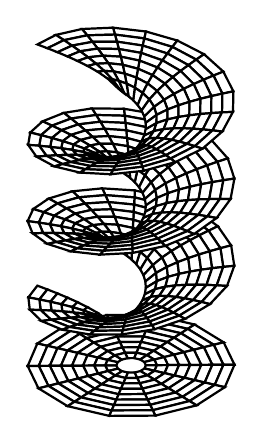
\begin{tikzpicture}[scale=2]
    \begin{axis}[
        axis lines=none,
        axis equal image,
        trig format plots=rad,
        z buffer=sort]
   \addplot3 [
        surf,
        domain=1:7,
        domain y=-pi:pi,
        samples=9,
        samples y=15,
        shader=flat,
        draw=black,
        fill=white
        ]
    ({x*cos(y)},{x*sin(y)},{-12});
   \addplot3 [
        surf,
        domain=1:7,
        samples=9,
        samples y=60,
        shader=flat,
        draw=black,
        fill=white,
        domain y=-3*pi:3*pi
        ]
    ({x*cos(y)},{x*sin(y)},{ln(x)+ y});
    \end{axis}
  \end{tikzpicture}




	      This map \textit{should} be local homeomorphism, but this is false in the Zariski topology. There do not exist nonempty open subsets $V$ and $U$ such that $x \to x^n$ maps $V$ isomorphically onto $U$. The theory of \'etale coverings will give us a good notion of covering which we will use to define the analog of universal coverings
\end{itemize}

The \'etale topology will provide a solution for the problems we have with both cohomology and fundamental groups. The \'etale topology is not a topology in the classical sense, but a category equipped with a notion of covering (in the sense of point-set topology). The analog of open sets of a scheme $X$ will be so called \'etale morphisms $U \to X$. \'Etale morphisms are the natural analogs of local homeomorphisms in scheme theory, so they provide a finer topology than the Zarisiki topology, giving rise to a better sheaf theory. Furthermore, surjective \'etale morphisms share a lot of formal properties with covering spaces, allowing us to define the \'etale fundamental group $\pi_1^{\et}$.



Riemann Hypothesis:
\begin{align}
	\zeta(s) = \sum_{n \ge 0} \frac{1}{n^s} \\
	\zeta(\lambda) = 0 nontrivial \implies Re(\lambda) = \frac{1}{2}
\end{align}

Dedekind, Artin, Hasse:
$R$ dedekind domain:
\[
	\zeta_R(s) = \sum_{I \subset R} \frac{1}{N(I)^s}, N(I) =\#R/I
\]

Special case:
\begin{align}
	R = \F_p[T] \iff \mathbb{A}_{\F_p}^1 = \Spec\F_p[T] \\
	\zeta_R(s) = \prod_{\pi irred}(\frac{1}{1-N\pi^{-s}} = \exp(\sum_{n \ge 1} \# X(\F_{p^n})\frac{T^n}{n}
\end{align}

Weil studies: $Z(X,T)$, $X/F$


  \chapter{Sites, Sheaves and Grothendieck Topoi}
  Much of modern geometry can be formulated in the language of sheaves. Sheaves are data that are given on a topological space that may be glued. One may more generally define sheaves on a category equipped with a so-called Grothendieck topology. A sheaf is a geometric gadget that relates local data (say, on a topological space) to global data. Sheaf theory gives us tools to systematically analyse local-global phenomena which are fundamental in geometry and topology.

\begin{construction}\label{def:opens}
  Let $X$ be a topological space. The open sets of $X$ are partially ordered by inclusion: \[V \le W \quad \text{iff} \quad V \subseteq W.\]
  We may thus consider the category of open sets of $X$, denoted by $\Op(X)$.
\end{construction}
A key observation is the following: In the category $\Op(X)$ pullbacks correspond to intersections and pushouts correspond to unions. By the definition of topological space, this means that $\Op(X)$ has finite pullbacks and arbitrary pushouts.

% TODO: replace res with id

\begin{definition}[Presheaves] 
  Let $X$ be a topological space. A \textit{presheaf of sets} $\mathcal{F}$  is a map which assings
  \begin{itemize}
    \item to each open subset $U$ of $X$ a set $\mathcal{F}(U)$. We call the elements of $\mathcal{F}(U)$ the \textit{sections of $\mathcal{F}$ over $U$}.
    \item to each inclusion of open sets $U \subseteq V$ a \textit{restriction map}
    \[i_*: \mathcal{F}(V) \longrightarrow\mathcal{F}(U).\]
  \end{itemize}
    The restriction maps need to have the following properties: 
    \begin{itemize}
      \item The restriction along the identity $V \subseteq V$ is the identity, so 
            \[id_* = id.\]
      \item For two inclusions $U \subseteq V \subseteq W$, the restricion maps adhere to the identity 
            \[res_{W\kern-0.1em , V}\ \circ\ res_{V\kern-0.1em , U} = res_{W\kern-0.1em , U}.\]
    \end{itemize}
  One may more slickly define a presheaf as a functor $\mathcal{F}: \Op(X)^{\op}\longrightarrow \Set$. To supress notation we will write $s|_V$ instead of $res_{V\kern-0.1em , U}(s).$ Here $s$ is a section over $U$.\\
\end{definition}
\begin{definition}[Sheaves]
  A presheaf $\mathcal{F}$ is a \textit{sheaf} if one can uniquely glue sections. Precisely, this means:
  \begin{enumerate}
    \item For an open set $U$, an open cover $\{U_i\}_{\indexset{i}{I}}$ of $U$ and $s, t \in \mathcal{F}(U)$, if $s|_{U_i} = t|_{U_i}$ for all $i \in I$, then $s = t$.
    \item For an open set $U$, an open cover $\{U_i\}_{\indexset{i}{I}}$ of $U$ and a family of sections
    \[\{s_i \in \mathcal{F}(U_i)\}_{\indexset{i}{I}},\]
     if $s_i|_{U_i \cap U_j} = s_j|_{U_i \cap U_j}$ for all $i,j \in I$, then there exists a section $s \in \mathcal{F}(U)$ such that $s|_{U_i} = s_i$ for all $i \in I$.
  \end{enumerate}
  In words this says that if we have a a cover $\{U_i\}$ of $U$ and a family of sections $\{s_i\}$ which agree on all intersections, we may glue these sections to a section over $U$. Moreover, this section is unique.
\end{definition}

Let $X$ be a topological space and $B$ a base for its topology. It is sometimes convenient to give a sheaf on a base instead of the topology.

% TODO: Examples: constant sheaves, sheaves of rings
The definition for presheaves and sheaves are given almost entirely in categorical language. The notion of presheaf on a category $C$ is readily defined as a functor 
\[\mathcal{F}: C^{\op}\longrightarrow \Set.\]
The missing piece is the notion of a covering in arbitrary categories.. To motivate the definition of a Grothendieck topology, we review the proerties of coverings in the language introduced in Definition \ref{def:opens}.
 \begin{enumerate}
  \item The identity $U \to U$ is an open cover of $U$.
  \item Coverings are stable under composition. Precisely this means: Given a covering \\$\{U_i \to U\}_{i \in I}$ and for each $U_i$ a covering $\{V_{ij} \to U_i\}_{j \in J}$, the composition
        \[\{V_{ij} \to U\}\]
        should be a covering of $U$.
   \item  Coverings are stable under pullback: If we have an inclusion $V \hookrightarrow U$ and a covering $\{U_i \to U\}$, the open sets $\{U_i \times_U V\}$ cover $V$ with the induced projection maps:
   % https://q.uiver.app/?q=WzAsNCxbMCwwLCJcXHtVX2kgXFx0aW1lc19VIFZcXH0iXSxbMCwxLCJWIl0sWzEsMCwiXFx7VV9pXFx9Il0sWzEsMSwiVSJdLFswLDFdLFswLDJdLFsyLDNdLFsxLDMsIiIsMCx7InN0eWxlIjp7InRhaWwiOnsibmFtZSI6Imhvb2siLCJzaWRlIjoidG9wIn19fV1d
      \[\begin{tikzcd}
      	{\{U_i \times_U V\}} & {\{U_i\}} \\
      	V & U.
      	\arrow[from=1-1, to=2-1]
      	\arrow[from=1-1, to=1-2]
      	\arrow[from=1-2, to=2-2]
      	\arrow[hook, from=2-1, to=2-2]
      \end{tikzcd}\]
      Here the fiber product may often be interpreted as the intersection.
\end{enumerate}
\begin{definition}[bases for Grothendieck topologies]
  
\end{definition}

\begin{example}
  We obtain a sheaf on $\R^n$ by associating to any open set $U\subseteq \R^n$ the set \[C(U) = \{f: U \to \R\}\]. The restriction maps are the usual ones. The other properties are also clear.
\end{example}
\begin{example}
  Let $X$ be a topological space. For any abelian group $A$ there is the so called \textit{constant sheaf} $X_A$. To any open set $U \subseteq X$ associate the set \[X_A(U) = \{f: U \to A | f \text{ is locally constant.} \}\]
\end{example}

\section{Maps of sheaves}
Since sheaves are presheaves, we define a map of sheaves $\varphi: \mathcal{F} \to \mathcal{G}$ as a natural transformation $\mathcal{F} \to \mathcal{G}$ between functors. Explicitly this natural transformation consists of a group homomorphism $\varphi_U: \mathcal{F}(U) \to \mathcal{G}(U)$ for each $U \in X$ that is compatible with the restrictions in the sense that the following diagram commutes:

% https://q.uiver.app/?q=WzAsNCxbMCwwLCJcXG1hdGhjYWx7Rn0oVikiXSxbMCwxLCJcXG1hdGhjYWx7Rn0oVSkiXSxbMSwwLCJcXG1hdGhjYWx7R30oVikiXSxbMSwxLCJcXG1hdGhjYWx7R30oVSkiXSxbMCwxLCJyZXNfe1YsVX0iLDJdLFswLDIsIlxcdmFycGhpX1YiXSxbMiwzLCJyZXNfe1YsVX0iXSxbMSwzLCJcXHZhcnBoaV9VIl1d
\[\begin{tikzcd}
	{\mathcal{F}(V)} & {\mathcal{G}(V)} \\
	{\mathcal{F}(U)} & {\mathcal{G}(U)}
	\arrow["{res_{V,U}}"', from=1-1, to=2-1]
	\arrow["{\varphi_V}", from=1-1, to=1-2]
	\arrow["{res_{V,U}}", from=1-2, to=2-2]
	\arrow["{\varphi_U}", from=2-1, to=2-2]
\end{tikzcd}\]

Let $\varphi : \mathcal{F} \to \mathcal{G}$ be a morphism sheaves of abelian groups on $X$. The sheaf kernel of the map $\varphi$ is the presheaf $U \mapsto ker(\varphi)$. The sheaf condition on $\mathcal{G}$ ensures that this is in fact a sheaf.



There are a number of properties of sheaves which are important for applications. These properties govern the behavior of the cohomology.

\begin{definition}
  A sheaf is called
  \begin{enumerate}
    \item flabby if the restriction maps are surjective,
    \item soft if any section over a closed subset can be extended to a global section,
    \item acyclic if the higher cohomology of the sheaf vanishes. 
  \end{enumerate} 
\end{definition}

\section{The \'Etale site of a Scheme}
%\section{Sheaf Semantics}
%It is possible to interpret intuitionistic first-order logic in an arbitrary topos. In the case of sheaves, this is done using the following rules

  \chapter{Axiomatic Cohesion}
  The notion of cohesion is supposed to be formalise what it means for a category $\mathcal{E}$ to be a category of spaces consisting of basic shapes of a category $\mathcal{S}$.
In defining cohesion, Lawvere was guided by the central example of topological spaces and sets. We will outline this example before giving the abstract defintion of cohesion.\\

\section{The cohesion of topological spaces}
Let $\Top$ and $\Set$ denote the category of locally connected topological spaces\footnote{The construction does not technically work for the category of \textit{all} topological spaces, but it is fine to ignore this technicality.} and sets respectively. There is the evident forgetful functor from $\Top$ to $\Set$, which we will denote by $\Gamma$. It assigns to each topological space $X$ the underlying set $\Gamma(X)$. There are also two functors $\Disc$ and $\CoDisc$, going from $\Set$ to $\Top$. The functor $\Disc$ assigns to a set $S$ the topological space $\Disc(S)$ with underlying set $S$ and the discrete topology, while $\CoDisc(S)$ is the space with the trivial topology. Lastly, there is also a functor $\Pi_0$ which takes a topological space to its set of connected components.
\begin{proposition}
  The functors described above form an adjoint quadruple \[\Pi_0 \dashv\ \Disc \dashv\ \Gamma \dashv\ \CoDisc.\]
\end{proposition}
\begin{proof}
  Let $S$ be a set and consider a set function $f: S \to \Gamma(X)$. Since any subset of $\Disc(S)$ is open, there exists a continuous function $\tilde{f}: \Disc(S) \to X$ such that the underlying set function is $f$. Conversely, any continuous function $\tilde{f} : \Disc(S) \to X$ gives rise to a set function $ f: S \to \Gamma(X)$. These assignments are clearly inverse to each other. (Naturality missing from proof). This shows that $\Disc \dashv\ \Gamma$.\\
  Next, for $g: X \to \CoDisc(S)$ a continous function, continuity just means that that $g^{-1}(S)$ is open since the only open subsets of $\CoDisc(S)$ are $\varnothing$ and $S$.
  But $g^{-1}(S)$ is just $X$. This implies that any set function from $\Gamma(X)$ to $S$ gives rise to a continuous function from $X$ to $\CoDisc(S)$. This shows that $\Gamma \dashv\ \CoDisc$.\\
  Finally, any continuous function into a discrete space must be locally constant, which means $\Hom(\Pi_0(X), S) \simeq \Hom(X, \Disc(S))$. This proves the last adjunction
\end{proof}

\section{Axiomatic Cohesion}
\section{Cohesion for gros Topoi}
\section{Cohesion for petit Topoi}
\section{WIP/Notes}
Cohesion is usually formulated in the "gros" perspective. I will now try to elaborate on a "petit" cohesion.
Let $X$ be a topological space. The global sections functor $\Gamma$ takes any open set $U \subset X$ to its underlying set. This can be seen as a sort of trivial structure sheaf. For any set $S$, there is an associated constant sheaf $\Delta(S)$. It takes an open set $U$ to the set of continuous functions $\{U \to \Disc(S)\}$

  \chapter{Cohomology in Topology}
  \begin{theorem}
  If $X$ is an irreducible topological space and $\Sh{F}$ is a constant sheaf, then $H^r(X, \Sh{F})$ for all $r>0$.
\end{theorem}
\begin{proof}
  Since any open set $U \subseteq X$ is connected, $\Sh{F}(U) = G$ if $\Sh{F}$ is the constant sheaf defined by the group $G$ and $U$ is nonempty. This means that $\Sh{F}$ is flasque, hence $H^r(X, \Sh{F})$ for all $r>0$.
\end{proof}
It follows that constant sheaves on varieties have no higher cohomology. The reason ist that there are not enough open sets in the Zariski topology. This was the reason for defining the \'etale topology. We will now see how the \'etale topology yields good cohomological results

As we have seen, sheaves relate the local and global information one has on a given topological space $X$. In a sense sheaf cohomology measures how much more information we gain when we go from global to local. For example, consider the sheaf of local sections of the covering space $\pi : X \to S^1$.

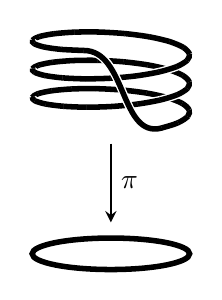
\begin{tikzpicture}[declare function={f(\x)=0.2*sin(\x)+\x/1000;},
  rubout/.style={/utils/exec=\tikzset{rubout/.cd,#1},
  decoration={show path construction,
       curveto code={
        \draw [white,line width=\pgfkeysvalueof{/tikz/rubout/line width}+2*\pgfkeysvalueof{/tikz/rubout/halo}] 
         (\tikzinputsegmentfirst) .. controls
         (\tikzinputsegmentsupporta) and (\tikzinputsegmentsupportb)  ..(\tikzinputsegmentlast); 
        \draw [line width=\pgfkeysvalueof{/tikz/rubout/line width},shorten <=-0.1pt,shorten >=-0.1pt] (\tikzinputsegmentfirst) .. controls
         (\tikzinputsegmentsupporta) and (\tikzinputsegmentsupportb) ..(\tikzinputsegmentlast);  
       }}},rubout/.cd,line width/.initial=2pt,halo/.initial=0.5pt]
  \draw[rubout={line width=2pt,halo=0.5pt},decorate] 
    plot[variable=\x,domain=-50:970,samples=55,smooth] ({cos(\x)},{f(\x)}) to[out=0,in=195] cycle;
  \draw[line width=2pt] (0,-2) arc(-90:270:1cm and 0.2cm);
  \draw[thick,-stealth]  (0,-0.4) -- (0,-1.4) node[midway,right]{$\pi$};
 \end{tikzpicture} 

There is no global section $s: S^1 \to X$ but locally, the set of sections $\{s: U \to \pi^{-1}(U) | \pi \circ s = id$ is a set with three elements.

Let $X$ be a topological space. A theorem of algebraic topology says that for any abelian group $A$, the cohomology group $H^1(X,A)$ with coefficients in $A$ is isomorphic to the abelianisation of the fundamental group $\pi_1(X)$

  \chapter{\'Etale Cohomology}
  The \'etale cohomology of a scheme was defined by Alexandre Grothendieck, Michael Artin and Jean-Luis Verdier in the late 50's. Andr\'e Weil had conjectured the existence of a cohomology theory for varieties over finite fields, from which his famous Weil conjectures could be deduced.

\section{\'Etale Morphisms}

\subsubsection{Local homeomorphisms}
In topology, a continuous map $f: X \to Y$ is called a local homeomorphism if $f$ restricts to a homeomorphism around any point $x \in X$. More precisely, for any point $x \in X$ there is a neighborhood $U$ of $x$ such that $f(U)$ is open in $Y$ and $p|_U: U \to p(U)$ is a homeomorphism. In this situation one also says that $X$ is an \'etale space over $Y$.
In the case of manifolds, this concept is easy to picture, since locally a manifold looks like $\mathbb{R}^n$ for some $n \in \mathbb{N}$. In the case of schemes, however, this is trickier.

\subsubsection{\'Etale morphsims of nonsingular varieties}
For varieties defined over an algebraically closed field $k$, one may use a formalism in direct analogy to smooth manifolds to define \'etale morphsims, namely the formalism of tangent spaces. However, instead of defining the tangent space at a point $p \in X$ analytically, we define it algebraically.

\subsubsection{\'Etale morphisms of affine schemes}
\begin{definition}
  A morphism $f: Y \to X$ is called an \'etale morphism if for every $y \in Y$ there exist open affine neighborhoods $V = spec B$ of $y$ and $Y = spec A$ of $f(y)$ such that 
  \[B = A[x_1, \dots, x_n]/(P_1, \dots, P_n)\]
  and $det(\partial P_i /\partial T_j)$ is a unit in $B$.
\end{definition}
This is not the standard definition of \'etale morphisms, but it is equivalent and according to the author the most intuitive.

\begin{proposition}
  The composite of two \'etale morphisms and base change of an \'etale morphims are \'etale.
\end{proposition}

Computing sheaf cohomology on a topological space using the formalism of derived functors is often unfeasable. Calculations are often done using Cech cohomology. The same is possible for \'etale cohomology. The definition of Cech cohomology for \'etale sheaves works with basically no modifications.
\section{\'Etale sheaves}
Examples of \'Etale sheaves:

The structure sheaf $\mathcal{O}_{X_{\text{\'et}}}(U) = \Gamma(U, \mathcal{O}_U)$
\par
Representables $\mathcal{F}: \mathsf{Et}/X \to \Set , \mathcal{F}(U) = \Hom_X(U,Z)$ for any $X$-scheme $Z$. In particular this means that the \'etale topology is subcanonical.
\par

It is a theorem that any category of sheaves on a site (in particular a topological space) is an elementary topos. As such it carries a lot of structure


  \chapter{Conclusion}
  \section*{}
conclusion bla bla

  \appendix
  \chapter{Review of categorical notions}
  \section{Categories, Functors and Natural Transformations}

\section{Diagrams, Cones, Limits and Colimits}
  Let $J$ be a small category (often called index category). A diagram $D$ of shape $J$ in $C$ is a functor $D: J \to C$. A cone over $D$ is an object $A$ with morphsism $\varphi_X: A \to D(X)$ for every object $X \in J$ such that for every morphism $f: X \to Y$ in $J$ the diagram 
  % https://q.uiver.app/?q=WzAsNCxbMSwwLCJBIl0sWzAsMSwiRChYKSJdLFsxLDJdLFsyLDEsIkQoWSkiXSxbMCwxLCJcXHZhcnBoaV9YIiwyXSxbMCwzLCJcXHZhcnBoaV9ZIl0sWzEsMywiRChmKSJdXQ==
\[\begin{tikzcd}
	& A \\
	{D(X)} && {D(Y)} \\
	& {}
	\arrow["{\varphi_X}"', from=1-2, to=2-1]
	\arrow["{\varphi_Y}", from=1-2, to=2-3]
	\arrow["{D(f)}", from=2-1, to=2-3]
\end{tikzcd}\]
  commutes.

\section{Adjunctions}
  \chapter{The definition of a Scheme}
  asdf

  \bibliographystyle{plain}
  \bibliography{refs}
\end{document}